\chapter{Results}%
\label{sec:results}

At ICHEP 2018 a result of the VH{(bb)} analysis was shown in which the Standard Model Higgs boson
search at $\sqrt{S}= 13$~TeV yielded an excess with an observed statistical significance of 4.9
standard deviations and a calculated expected significance of 4.3 standard
deviations~\cite{ATLAS-CONF-2018-036}. Further combining this result with the other Higgs production
channels and results from Run 1 yielded an observed significance of 5.4 standard deviations with an
expected significance of 5.5 standard deviations. This is above threshold for what is considered a
discovery of the process.

\section{Re-weighting of single top processes}

As mentioned in Chapter~\ref{sec:analysis} a bespoke BDT re-weighting algorithm was studied to aim to
quantify the difference between two generators of single top processes. The variables relevant to the
$Wt$ process are split up into four different subspaces which are each trained on separately. The
spaces are defined as follows in table~\ref{tab:subspace}. Datasets used to train these algorithms are listed in Appendix~\ref{app:datasets}.
\begin{table}[h]
  \centering
  \begin{tabular}{lC{5em}C{5em}} 
    &  2 b-jets &  $\leq$ 1 b-jets \\
    \midrule
    2 jets & subspace 1 & subspace 2 \\ [5ex]
    \midrule
    3 jets & subspace 3 & subspace 4 \\ [5ex]
    \bottomrule
  \end{tabular}
  \caption{The four subspaces that events were split up into before training.}%
  \label{tab:subspace}
\end{table}
The variables used for the training are shown in Appendix~\ref{app:feat}. They
differ for three jet and two jet samples but are unchanged by the number of
b-jets. Two-fold cross validation was used to promote generalisation.

Figures~\ref{fig:mindphi-res},~\ref{fig:mbb-res},~\ref{fig:dR-res},~and~\ref{fig:pt3-res} show one
dimensional projects of some of the training variables. The distribution that was to be re-weighted is
shown before (black) and after (blue) the weights are applied. A comparison can be made between the
overall shape of these distributions and the target distribution (also plotted). It can be seen in
these figures that, whilst performance varies between variables, the BDT re-weighter consistently
results in a shape that closely matches the target distribution. It should be noted that observing one
dimensional projections does not give a complete comparison of the shapes of multi-dimensional
distributions. It is also noted that more work needs to be completed before these results can be turned
into a proper systematic uncertainty.

\begin{figure}[h]
  \centering
  \includegraphics[scale=0.75]{Wt_2j_b1b2are5/dPhiLBmin/folding_rw_all_dPhiLBmin}
  \caption{Plot of $\min(\Delta\phi(\ell, jet))$ in the sub-space where there
    are two jets that are both b-jets.}%
  \label{fig:mindphi-res}
\end{figure}

\begin{figure}[ht]
  \centering
  \includegraphics[scale=0.75]{Wt_3j_b1b2are5/mBB/folding_rw_all_mBB}
  \caption{Plot of $m_{jj}$ in the sub-space where there are three
    jets and exactly two are b-jets.}%
  \label{fig:mbb-res}
\end{figure}

\begin{figure}[h]
  \centering
  \includegraphics[scale=0.75]{Wt_3j_b1b2are5/dRBB/folding_rw_all_dRBB}
  \caption{Plot of $\Delta R(jet_1, jet_2)$ in the sub-space where there are
    three jets and exactly two are b-jets.}%
  \label{fig:dR-res}
\end{figure}

\begin{figure}[h]
  \centering
  \includegraphics[scale=0.75]{Wt_3j_b1b2not5/pTJ3/folding_rw_all_pTJ3}
  \caption{Plot of $p^{jet3}_{T}$ in the sub-space where there are three
    jets of which, the leading and sub-leading jets are not both b-jets
    (one is allowed).}%
  \label{fig:pt3-res}
\end{figure}

%\begin{figure}[ht]
%  \centering
%  \includegraphics[scale=0.75]{Wt_2j_b1b2are5/dPhiLBmin/folding_rw_all_dPhiLBmin}
%  \caption{Plot of $min(\Delta\phi(\ell, jet))$ in the sub-space where there
%    are two jets that are both b-jets.}
%\end{figure}
%
%\begin{figure}[ht]
%  \centering
%  \includegraphics[scale=0.75]{Wt_2j_b1b2are5/dPhiVBB/folding_rw_all_dPhiVBB}
%  \caption{Plot of $\Delta\phi(V, H))$ in the sub-space where there are two
%    jets that are both b-jets.}
%\end{figure}
%
%\begin{figure}[ht]
%  \centering
%  \includegraphics[scale=0.75]{Wt_2j_b1b2are5/dRBB/folding_rw_all_dRBB}
%  \caption{Plot of $\Delta R(jet_1, jet_2) $ in the sub-space where there are
%    two jets that are both b-jets.}
%\end{figure}
%
%\begin{figure}[ht]
%  \centering
%  \includegraphics[scale=0.75]{Wt_2j_b1b2are5/dYWH/folding_rw_all_dYWH}
%  \caption{Plot of $\Delta Y(W, H)$ in the sub-space where there are twojets
%    that are both b-jets.}
%\end{figure}
%
%\begin{figure}[ht]
%  \centering
%  \includegraphics[scale=0.75]{Wt_2j_b1b2are5/mBB/folding_rw_all_mBB}
%  \caption{Plot of $m_{jj}$ in the sub-space where there are two
%    jets that are both b-jets.}
%\end{figure}
%
%\begin{figure}[ht]
%  \centering
%  \includegraphics[scale=0.75]{Wt_2j_b1b2are5/MET/folding_rw_all_MET}
%  \caption{Plot of $E^{miss}_{T}$ in the sub-space where there are two
%    jets that are both b-jets.}
%\end{figure}
%
%\begin{figure}[ht]
%  \centering
%  \includegraphics[scale=0.75]{Wt_2j_b1b2are5/Mtop/folding_rw_all_Mtop}
%  \caption{Plot of $m_{top}$ in the sub-space where there are two
%    jets that are both b-jets.}
%\end{figure}
%
%\begin{figure}[ht]
%  \centering
%  \includegraphics[scale=0.75]{Wt_2j_b1b2are5/mTW/folding_rw_all_mTW}
%  \caption{Plot of $m^{W}_{T}$ in the sub-space where there are two
%    jets that are both b-jets.}
%\end{figure}
%
%\begin{figure}[ht]
%  \centering
%  \includegraphics[scale=0.75]{Wt_2j_b1b2are5/pTB1/folding_rw_all_pTB1}
%   \caption{Plot of $p^{jet1}_{T}$ in the sub-space where there are two
%    jets that are both b-jets.}
%\end{figure}
%
%\begin{figure}[ht]
%  \centering
%  \includegraphics[scale=0.75]{Wt_2j_b1b2are5/pTB2/folding_rw_all_pTB2}
%  \caption{Plot of $p^{jet2}_{T}$ in the sub-space where there are two
%    jets that are both b-jets.}
%\end{figure}
%
%\begin{figure}[ht]
%  \centering
%  \includegraphics[scale=0.75]{Wt_2j_b1b2are5/pTV/folding_rw_all_pTV}
%  \caption{Plot of $p^{V}_{T}$ in the sub-space where there are two
%    jets that are both b-jets.}
%\end{figure}
%
%%-----------------------------------------------------------------------------
%
%\begin{figure}[ht]
%  \centering
%  \includegraphics[scale=0.75]{Wt_2j_b1b2not5/dPhiLBmin/folding_rw_all_dPhiLBmin}
%  \caption{Plot of $min(\Delta\phi(\ell, jet))$ in the sub-space where there are
%    two jets and they are not both b-jets (one b-jet is allowed).}
%\end{figure}
%
%\begin{figure}[ht]
%  \centering
%  \includegraphics[scale=0.75]{Wt_2j_b1b2not5/dPhiVBB/folding_rw_all_dPhiVBB}
%  \caption{Plot of $\Delta\phi(V, H))$ in the sub-space where there are two jets
%  and they are not both b-jets (one b-jet is allowed).}
%  
%\end{figure}
%
%\begin{figure}[ht]
%  \centering
%  \includegraphics[scale=0.75]{Wt_2j_b1b2not5/dRBB/folding_rw_all_dRBB}
%  \caption{Plot of $\Delta R(jet_1, jet_2)$ in the sub-space where there are
%    two jets and they are not both b-jets (one b-jet is allowed).}
%\end{figure}
%
%\begin{figure}[ht]
%  \centering
%  \includegraphics[scale=0.75]{Wt_2j_b1b2not5/dYWH/folding_rw_all_dYWH}
%  \caption{Plot of $\Delta Y(W, H)$ in the sub-space where there are two jets
%  and they are not both b-jets (one b-jet is allowed).}
%\end{figure}
%
%\begin{figure}[ht]
%  \centering
%  \includegraphics[scale=0.75]{Wt_2j_b1b2not5/mBB/folding_rw_all_mBB}
%  \caption{Plot of $m_{jj}$ in the sub-space where there are two jets
%  and they are not both b-jets (one b-jet is allowed).}
%\end{figure}
%
%\begin{figure}[ht]
%  \centering
%  \includegraphics[scale=0.75]{Wt_2j_b1b2not5/MET/folding_rw_all_MET}
%  \caption{Plot of $E^{miss}_{T}$ in the sub-space where there are two jets
%  and they are not both b-jets (one b-jet is allowed).}
%\end{figure}
%
%\begin{figure}[ht]
%  \centering
%  \includegraphics[scale=0.75]{Wt_2j_b1b2not5/Mtop/folding_rw_all_Mtop}
%  \caption{Plot of $m_{top}$ in the sub-space where there are two jets
%  and they are not both b-jets (one b-jet is allowed).}
%\end{figure}
%
%\begin{figure}[ht]
%  \centering
%  \includegraphics[scale=0.75]{Wt_2j_b1b2not5/mTW/folding_rw_all_mTW}
%  \caption{Plot of $m^{W}_{T}$ in the sub-space where there are two jets
%  and they are not both b-jets (one b-jet is allowed).}
%\end{figure}
%
%\begin{figure}[ht]
%  \centering
%  \includegraphics[scale=0.75]{Wt_2j_b1b2not5/pTB1/folding_rw_all_pTB1}
%  \caption{Plot of $p^{jet1}_{T}$ in the sub-space where there are two jets
%  and they are not both b-jets (one b-jet is allowed).}
%\end{figure}
%
%\begin{figure}[ht]
%  \centering
%  \includegraphics[scale=0.75]{Wt_2j_b1b2not5/pTB2/folding_rw_all_pTB2}
%  \caption{Plot of $p^{jet2}_{T}$ in the sub-space where there are two jets
%  and they are not both b-jets (one b-jet is allowed).}
%\end{figure}
%
%\begin{figure}[ht]
%  \centering
%  \includegraphics[scale=0.75]{Wt_2j_b1b2not5/pTV/folding_rw_all_pTV}
%  \caption{Plot of $p^{V}_{T}$ in the sub-space where there are two jets
%  and they are not both b-jets (one b-jet is allowed).}
%\end{figure}
%
%%-------------------------------------------------------------------------------
%
%%-------------------------------------------------------------------------------
%
%\begin{figure}[ht]
%  \centering
%  \includegraphics[scale=0.75]{Wt_3j_b1b2are5/dPhiLBmin/folding_rw_all_dPhiLBmin}
%  \caption{Plot of $min(\Delta\phi(\ell, jet))$ in the sub-space where there
%    are three jets and exactly two are b-jets.}
%\end{figure}
%
%\begin{figure}[ht]
%  \centering
%  \includegraphics[scale=0.75]{Wt_3j_b1b2are5/dPhiVBB/folding_rw_all_dPhiVBB}
%  \caption{Plot of $\Delta\phi(V, H))$ in the sub-space where there are three
%    jets and exactly two are b-jets.}
%\end{figure}
%
%\begin{figure}[ht]
%  \centering
%  \includegraphics[scale=0.75]{Wt_3j_b1b2are5/dRBB/folding_rw_all_dRBB}
%  \caption{Plot of $\Delta R(jet_1, jet_2)$ in the sub-space where there are
%    three jets and exactly two are b-jets.}
%\end{figure}
%
%\begin{figure}[ht]
%  \centering
%  \includegraphics[scale=0.75]{Wt_3j_b1b2are5/dYWH/folding_rw_all_dYWH}
%  \caption{Plot of $\Delta Y(W, H)$ in the sub-space where there are three
%    jets and exactly two are b-jets.}
%\end{figure}
%
%\begin{figure}[ht]
%  \centering
%  \includegraphics[scale=0.75]{Wt_3j_b1b2are5/mBB/folding_rw_all_mBB}
%  \caption{Plot of $m_{jj}$ in the sub-space where there are three
%    jets and exactly two are b-jets.}
%\end{figure}
%
%\begin{figure}[ht]
%  \centering
%  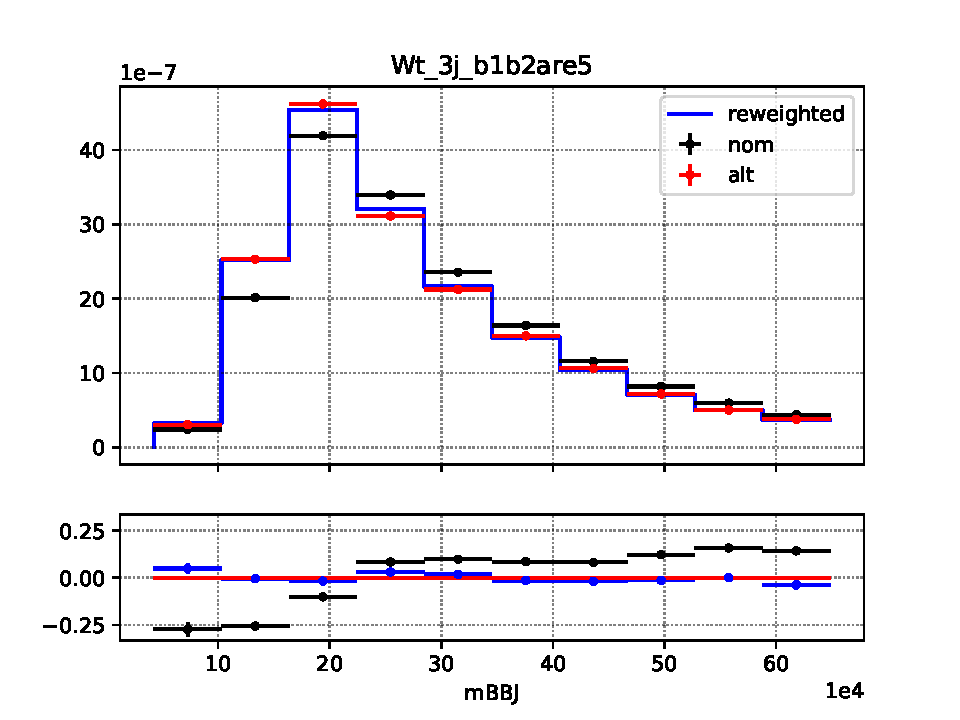
\includegraphics[scale=0.75]{Wt_3j_b1b2are5/mBBJ/folding_rw_all_mBBJ}
%  \caption{Plot of $m_{jjj}$ in the sub-space where there are three
%    jets and exactly two are b-jets.}
%\end{figure}
%
%\begin{figure}[ht]
%  \centering
%  \includegraphics[scale=0.75]{Wt_3j_b1b2are5/MET/folding_rw_all_MET}
%  \caption{Plot of $E^{miss}_{T}$ in the sub-space where there are three
%    jets and exactly two are b-jets.}
%\end{figure}
%
%\begin{figure}[ht]
%  \centering
%  \includegraphics[scale=0.75]{Wt_3j_b1b2are5/Mtop/folding_rw_all_Mtop}
%  \caption{Plot of $m_{top}$ in the sub-space where there are three
%    jets and exactly two are b-jets.}
%\end{figure}
%
%\begin{figure}[ht]
%  \centering
%  \includegraphics[scale=0.75]{Wt_3j_b1b2are5/mTW/folding_rw_all_mTW}
%  \caption{Plot of $m^{W}_{T}$ in the sub-space where there are three
%    jets and exactly two are b-jets.}
%\end{figure}
%
%\begin{figure}[ht]
%  \centering
%  \includegraphics[scale=0.75]{Wt_3j_b1b2are5/pTB1/folding_rw_all_pTB1}
%  \caption{Plot of $p^{jet1}_{T}$ in the sub-space where there are three
%    jets and exactly two are b-jets.}
%\end{figure}
%
%\begin{figure}[ht]
%  \centering
%  \includegraphics[scale=0.75]{Wt_3j_b1b2are5/pTB2/folding_rw_all_pTB2}
%  \caption{Plot of $p^{jet2}_{T}$ in the sub-space where there are three
%    jets and exactly two are b-jets.}
%\end{figure}
%
%\begin{figure}[ht]
%  \centering
%  \includegraphics[scale=0.75]{Wt_3j_b1b2are5/pTJ3/folding_rw_all_pTJ3}
%  \caption{Plot of $p^{jet3}_{T}$ in the sub-space where there are three
%    jets and exactly two are b-jets.}
%\end{figure}
%
%\begin{figure}[ht]
%  \centering
%  \includegraphics[scale=0.75]{Wt_3j_b1b2are5/pTV/folding_rw_all_pTV}
%  \caption{Plot of $p^{V}_{T}$ in the sub-space where there are three
%    jets and exactly two are b-jets.}
%\end{figure}
%
%%------------------------------------------------------------------------------
%
%\begin{figure}[ht]
%  \centering
%  \includegraphics[scale=0.75]{Wt_3j_b1b2not5/dPhiLBmin/folding_rw_all_dPhiLBmin}
%  \caption{Plot of $min(\Delta\phi(\ell, jet))$ in the sub-space where there are
%    three jets of which, the leading and sub-leading jets are not both b-jets
%    (one is allowed).}
%  
%\end{figure}
%
%\begin{figure}[ht]
%  \centering
%  \includegraphics[scale=0.75]{Wt_3j_b1b2not5/dPhiVBB/folding_rw_all_dPhiVBB}
% \caption{Plot of $\Delta\phi(V, H))$ in the sub-space where there are three
%   jets of which, the leading and sub-leading jets are not both b-jets
%   (one is allowed).}
%\end{figure}
%
%\begin{figure}[ht]
%  \centering
%  \includegraphics[scale=0.75]{Wt_3j_b1b2not5/dRBB/folding_rw_all_dRBB}
%  \caption{Plot of $\Delta R(jet_1, jet_2)$ in the sub-space where there are
%    three jets of which, the leading and sub-leading jets are not both b-jets
%    (one is allowed).}
%\end{figure}
%
%\begin{figure}[ht]
%  \centering
%  \includegraphics[scale=0.75]{Wt_3j_b1b2not5/dYWH/folding_rw_all_dYWH}
%  \caption{Plot of $\Delta Y(W, H)$ in the sub-space where there are three
%    jets of which, the leading and sub-leading jets are not both b-jets
%    (one is allowed).}
%\end{figure}
%
%\begin{figure}[ht]
%  \centering
%  \includegraphics[scale=0.75]{Wt_3j_b1b2not5/mBB/folding_rw_all_mBB}
%  \caption{Plot of $m_{jj}$ in the sub-space where there are three
%    jets of which, the leading and sub-leading jets are not both b-jets
%    (one is allowed).}
%\end{figure}
%
%\begin{figure}[ht]
%  \centering
%  \includegraphics[scale=0.75]{Wt_3j_b1b2not5/Mtop/folding_rw_all_Mtop}
%  \caption{Plot of $m_{top}$ in the sub-space where there are three
%    jets of which, the leading and sub-leading jets are not both b-jets
%    (one is allowed).}
%\end{figure}
%
%\begin{figure}[ht]
%  \centering
%  \includegraphics[scale=0.75]{Wt_3j_b1b2not5/mTW/folding_rw_all_mTW}
%  \caption{Plot of $m^{W}_{T}$ in the sub-space where there are three
%    jets of which, the leading and sub-leading jets are not both b-jets
%    (one is allowed).}
%\end{figure}
%
%\begin{figure}[ht]
%  \centering
%  \includegraphics[scale=0.75]{Wt_3j_b1b2not5/pTB1/folding_rw_all_pTB1}
%  \caption{Plot of $p^{jet1}_{T}$ in the sub-space where there are three
%    jets of which, the leading and sub-leading jets are not both b-jets
%    (one is allowed).}
%\end{figure}
%
%\begin{figure}[ht]
%  \centering
%  \includegraphics[scale=0.75]{Wt_3j_b1b2not5/pTB2/folding_rw_all_pTB2}
%  \caption{Plot of $p^{jet2}_{T}$ in the sub-space where there are three
%    jets of which, the leading and sub-leading jets are not both b-jets
%    (one is allowed).}
%\end{figure}
%
%\begin{figure}[ht]
%  \centering
%  \includegraphics[scale=0.75]{Wt_3j_b1b2not5/pTJ3/folding_rw_all_pTJ3}
%  \caption{Plot of $p^{jet3}_{T}$ in the sub-space where there are three
%    jets of which, the leading and sub-leading jets are not both b-jets
%    (one is allowed).}
%\end{figure}
%
%\begin{figure}[ht]
%  \centering
%  \includegraphics[scale=0.75]{Wt_3j_b1b2not5/pTV/folding_rw_all_pTV}
%  \caption{Plot of $p^{V}_{T}$ in the sub-space where there are three
%    jets of which, the leading and sub-leading jets are not both b-jets
%    (one is allowed).}
%\end{figure}

